\documentclass{beamer}
%\documentclass[12pt,handout]{beamer}

\usepackage[T1]{fontenc}
\usepackage{ae,aecompl}
\usepackage{pgfpages}
\usepackage{graphicx}
\usepackage{hyperref}
\usepackage{tikz}
\usetikzlibrary{shapes,backgrounds}

%\setbeameroption{show only notes}
%\setbeameroption{show notes on second screen}
%\setbeameroption{show notes on second screen=bottom}

\usetheme{default}

\title{Graduate School}
\subtitle{What I Wish I Knew in Third Year}
\author[Ming-Ho Yee]{Ming-Ho Yee\\ \href{http://mhyee.com}{\texttt{mhyee.com}}}
\institute{University of Waterloo\\
Bachelor Software Engineering, 2014\\
MMath Candidate in Computer Science}
%\date{\today}
\date{September 18, 2014}

\begin{document}

\maketitle
\note[itemize]{%
  \item Introduce myself and the presentation
  \item Q \& A session at the end with professors
  \item Slides are online, with some extra links at the end
}

\section{Introduction}
\begin{frame}
  \frametitle{What This Presentation Is About}
  \begin{itemize}
      \item What I wish I knew in third year
      \item What I learned since third year
  \end{itemize}
  \vspace{1em}
  \begin{center}
    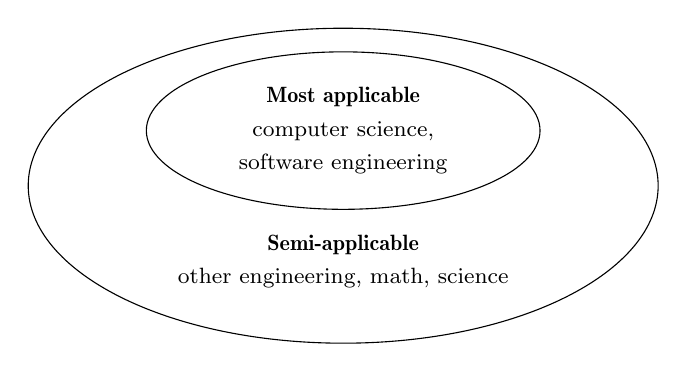
\begin{tikzpicture}
      \draw (0,0.7) ellipse (2.5cm and 1cm) node[align=center]
        {\textbf{\footnotesize Most applicable}\\
        {\footnotesize computer science,}\\
        {\footnotesize software engineering}};
      \draw (0,0) ellipse (4cm and 2cm) node[below=0.5cm, align=center]
        {\textbf{\footnotesize Semi-applicable}\\
        {\footnotesize other engineering, math, science}};
    \end{tikzpicture}
  \end{center}
\end{frame}
\note[itemize]{%
  \item Originally designed this for 3A SE
  \item This is the presentation I wish I had in third year
  \item I knew very little about grad school
  \item Learned on my own, and now sharing my knowledge
  \item This presentation is less applicable for other fields
}

\begin{frame}
  \frametitle{My Experiences}
  \begin{columns}[c]
    \column{0.5\linewidth}
    Research experiences:
    \begin{itemize}
      \item Undergrad: Co-op, URA, FYDP
      \item Now a graduate student in computer science
    \end{itemize}
    \column{0.4\linewidth}
    
\includegraphics[width=\linewidth]{images/uw-logo.png}
  \end{columns}
\end{frame}
\note[itemize]{%
  \item Caveat: I just started my graduate studies
  \item But I have some research experience from undergrad
  \item I've done research co-op, URA, and FYDP
  \item I applied to grad schools in Canada/US, including Waterloo
}

\begin{frame}
  \frametitle{My Experiences}
  \begin{columns}[c]
    \column{0.5\linewidth}
    Industry experiences:
    \begin{itemize}
      \item Telecommunications, web development startup
      \item Most recently: Visual C++ compiler at Microsoft
    \end{itemize}
    \column{0.4\linewidth}
    
\includegraphics[width=\linewidth]{images/vs-logo.png}
  \end{columns}
\end{frame}
\note[itemize]{%
  \item Also have industry experience
  \item Worked in telecom, two terms in a Rails startup with only two other devs
  \item Two terms (plus summer internship) with VS at Microsoft, most recently
        on their C++ compiler
  \item I think I have a pretty good idea of both sides
}

\section{Explaining Graduate School}
\begin{frame}
  \frametitle{Course-based Degree}
  \begin{itemize}
    \item Pay tuition and take courses (consume knowledge)
    \item Examples: law school, med school, MBA, MMath, MEng
  \end{itemize}
\end{frame}
\note[itemize]{%
  \item Definition: school after you have your bachelor's degree
  \item Need to clarify before going further: two kinds of grad school
  \item Course-based degree: you pay tuition and take courses
  \item You are a consumer of knowledge
  \item Examples: law school, med school, MBA, MMath (UW CS), MEng (UW ECE)
}

\begin{frame}
  \frametitle{Research-based Degree}
  \begin{itemize}
    \item Paid to do research (produce new knowledge)
    \item Examples: MMath, MASc, PhD
    \item
      \href{http://matt.might.net/articles/phd-school-in-pictures/}{%
        \color{blue}{See also Matt Might's illustrated guide to a Ph.D.}
      }
  \end{itemize}
  \vspace{2em}
  After this point, ``graduate school'' refers to \alert{research}.
\end{frame}
\note[itemize]{%
  \item Research-based degree: you are paid a salary to do research
  \item You are a producer of knowledge
  \item Matt Might (prof at University of Utah) has a nice little comic
  \item Examples: MMath (UW CS), MASc (UW ECE), PhD
  \item Note that at Waterloo, MMath is used for both course and thesis master's
        degrees
  \item In the US, ``master's'' typically means course-based
  \item But sometimes a US master's is earned en-route to a PhD
}

\section{Reasons for Graduate School}
\begin{frame}
  \frametitle{Reasons for Graduate School}
  \href{http://pgbovine.net/why-pursue-PhD.htm}{%
    \color{blue}{Philip Guo offers three practical reasons:}
  }
  \begin{itemize}
    \item Make a name for yourself
    \item Fail in a safe environment
    \item Choose from more jobs
  \end{itemize}
  \vspace{2em}
  In other words, ``trade money for freedom.''
\end{frame}
\note[itemize]{%
  \item There are many different reasons
  \item Many of them can be personal
  \item Philip Guo (professor at University of Rochester) offers three practical
        reasons
  \item Make a name for yourself, fail in a safe environment, choose from more
        jobs
  \item In other words, ``trade money for freedom''
}

\begin{frame}
  \frametitle{Make a Name for Yourself}
  \begin{itemize}
    \item Formulate, execute, and sell your ideas
    \item Entire process from start to finish, on your own
  \end{itemize}
\end{frame}
\note[itemize]{%
  \item Formulate, execute, and sell your ideas
  \item Come up with an idea, implement or test it, then write papers and give
        presentations
  \item It's your work
  \item ``On your own,'' but you get mentoring from peers and professors
  \item Note: startups are another way to do this
}

\begin{frame}
  \frametitle{Fail in a Safe Environment}
  \begin{itemize}
    \item Failure is an opportunity for growth
    \item Failure can inspire grit, tenacity, and perseverance
    \item Expected to fail repeatedly, without hurting career
  \end{itemize}
\end{frame}
\note[itemize]{%
  \item Grad school is uncertain and challenging
  \item There will be a lot of failure (ideas shot down, papers rejected, etc.)
  \item ``What doesn't kill you makes you stronger''
  \item Grit, tenacity, and perseverance
  \item These are good skills to have in any job
  \item In other jobs, failure may result in consequences (getting fired, not
        getting promoted, losing your startup, etc.)
  \item Though you don't necessarily need failure to develop these skills
}

\begin{frame}
  \frametitle{Choose From More Jobs}
  \begin{itemize}
    \item Co-op experiences makes us very employable at graduation
    \item A PhD can open even more opportunities
      \begin{itemize}
        \item Corporate research, academic research, teaching
      \end{itemize}
  \end{itemize}
  \vspace{2em}
  Trade money for freedom.
\end{frame}
\note[itemize]{%
  \item We are very employable after graduation
  \item Many of us get full-time offers by our last co-op term
  \item And if you don't have an offer, you still have job experience and
        interview skills
  \item But a PhD opens more doors for your career
  \item New opportunities are also different, and have more intellectual freedom
  \item Caveat: getting out of touch after you get your PhD
  \item Can maintain skills with internships
}

\begin{frame}
  \frametitle{Reasons Against Graduate School}
  You might not want to consider graduate school if you:
  \vspace{2em}

  \begin{itemize}
    \item like working in industry
    \item find it important to make a good salary now
  \end{itemize}
  \vspace{2em}

  Graduate school might not result in a higher salary later, either.
\end{frame}
\note[itemize]{%
  \item There are reasons to not go to graduate school
  \item If like working in industry or don't like research
  \item If it's important to make a good salary
  \item Salary can be 3 to 4 times lower in grad school
  \item Graduate degree might not result in a higher salary later
  \item It depends on the company and position: some don't care
  \item Another factor to consider is the time investment
  \item A master's might be worth it: the salary bump might be able to pay off
        the time investment
  \item But a PhD takes too long, and will cost you money
}

\section{Applying to Graduate School}
\begin{frame}
  \frametitle{Job Application for a Research Position}
  \begin{itemize}
    \item Apply 1 year before expected start
    \item Publications (research experience)
    \item Potential (to do research)
    \item Other qualities:
      \begin{itemize}
        \item \href{http://matt.might.net/articles/successful-phd-students/}{%
          \color{blue}{Perseverance, tenacity, cogency}
        }
      \end{itemize}
  \end{itemize}
\end{frame}
\note[itemize]{%
  \item Let's say you're sold and now want to apply for grad school
  \item You'll apply 1 year before you expect to start
  \item For SE students, this will be during your last co-op
  \item Can be difficult if you're not in Waterloo
  \item Application is a job application, so you'll need experience or potential
  \item Publications = experience
  \item Matt Might lists three qualities of successful PhD students
  \item Perseverance and tenacity: Getting a PhD is open-ended, uncertain, and
        full of rejection/failure
  \item Cogency: Ability to articulate ideas, in papers and presentations
}

\begin{frame}
  \frametitle{Research Experience}
  \begin{itemize}
    \item Work with different professors
    \item Opportunities:
      \begin{itemize}
        \item Co-op, URA, FYDP, SE 499
      \end{itemize}
  \end{itemize}
\end{frame}
\note[itemize]{%
  \item Working with different professors gives you multiple reference letters
  \item Opportunities: co-op, URA, FYDP, SE 499
  \item May have to go ``outside JobMine'' for research co-ops
  \item URA can be difficult, since it's on top of your course work
  \item Research experience is encouraged even if you're not sure about grad
        school
  \item Try something out, see if you like it, keep your options open
  \item If you don't do it, you're closing doors
  \item Easier to jump off the research path than jump onto it
}

\begin{frame}
  \frametitle{Letters of Recommendation}
  \begin{itemize}
    \item Need 2--3 letters
    \item Strong, academic references
      \begin{itemize}
        \item Professor you've done research with
      \end{itemize}
    \item ``Course'' letter
      \begin{itemize}
        \item Professor whose course you excelled in
      \end{itemize}
    \item Industry letter
      \begin{itemize}
        \item Demonstrated qualities appropriate for research
        \item Some programs won't accept these letters
      \end{itemize}
  \end{itemize}
\end{frame}
\note[itemize]{%
  \item 2--3 letters, depending on the program
  \item Best letter is the strong academic letter, from a prof you worked with
  \item Ideally you'd want 3, but 2 is OK
  \item Course letter is from a prof whose class you took and excelled in
  \item Good courses: small class, large open-ended project
  \item Industry letter from an employer who can write about your perseverance,
        tenacity, and cogency
  \item But note that some programs won't accept these letters
  \item Waterloo ECE will, but Waterloo CS will not
}

\begin{frame}
  \frametitle{Personal Statement}
  \begin{itemize}
    \item Convince admissions committee that you are a strong candidate
    \item Describe your research experience and interests
  \end{itemize}
\end{frame}
\note[itemize]{%
  \item Purpose is to convince admissions committee that you are a strong
        candidate
  \item Mostly you'll be writing about research experience and interests
  \item Other things: why you got into research, research plans, career plans
}

\begin{frame}
  \frametitle{Other Application Materials}
  \begin{itemize}
    \item Resume
    \item Grades
      \begin{itemize}
        \item May or may not be a cutoff
      \end{itemize}
    \item Graduate Record Examinations (GREs)
      \begin{itemize}
        \item Standardized test (similar to SATs)
        \item For US schools
      \end{itemize}
  \end{itemize}
\end{frame}
\note[itemize]{%
  \item The most important thing is research experience
  \item Importance of resume, grades, and GREs depends on the school
  \item Grade cutoff at Waterloo is 78\% (CS and ECE)
  \item US schools will use GPA, so you'll have to convert
  \item Study for GREs early, before you get too specialized in CS and rusty in
        basic math
  \item GRE scores are usually good for up to five years
  \item Also, grades \textit{are} relevant for scholarships
}

\section{Summary}
\begin{frame}
  \frametitle{\insertsection}
  \begin{itemize}
    \item What is graduate school?
      \begin{itemize}
        \item A job to do research: produce new knowledge
      \end{itemize}
    \item Reasons for graduate school?
      \begin{itemize}
        \item Make a name for yourself, fail in a safe environment, choose from
          more jobs
      \end{itemize}
    \item How to apply to graduate school?
      \begin{itemize}
        \item Get research experience, which gets you essay material and letters
      \end{itemize}
  \end{itemize}
\end{frame}
\note[itemize]{%
  \item There are three takeaway messages from this presentation
  \item Grad school is a job to do research, to produce new knowledge
  \item Three reasons for grad school: make a name for yourself, fail in a safe
        environment, choose from more jobs
  \item To apply, you'll need research experience
  \item If you're not sure and want to keep your options open, get research
        experience
}

\appendix
\begin{frame}
  \frametitle{Further Reading}
  \begin{itemize}
    \item \href{http://www.cs.cmu.edu/~harchol/gradschooltalk.pdf}{%
      \color{blue}{Applying to Ph.D. Programs in Computer Science}
    }
    \item \href{http://pgbovine.net/PhD-memoir.htm}{%
      \color{blue}{\textit{The Ph.D. Grind}}
    }
    \item \href{http://matt.might.net/articles/}{%
      \color{blue}{Matt Might's blog}
    }
    \item \href{http://pgbovine.net/phd.htm}{%
      \color{blue}{Philip Guo's articles}
    }
  \end{itemize}
\end{frame}
\note[itemize]{%
  \item ``Applying to Ph.D. Programs'' is written by a professor at CMU
  \item \textit{The Ph.D. Grind} is an ebook by Philip Guo about his PhD
        experience
}

\end{document}
